\documentclass[11pt,a4paper]{article}
\usepackage[utf8]{inputenc}
\usepackage{amsmath, amssymb, amsthm}
\usepackage{geometry}
\usepackage{graphicx}
\usepackage{booktabs}
\usepackage{hyperref}
\usepackage{xcolor}
\usepackage{empheq}
\usepackage{tikz}
\usetikzlibrary{positioning, arrows.meta}
\geometry{margin=1in}
\usepackage{algorithm}
\usepackage{algpseudocode}

\title{\textbf{Linear Regression}}
\author{\textbf{Nishanka Das} \\ 
Department of Computer Science \\ 
Ramakrishna Mission Vivekananda Centenary College, Rahara}
\date{\today}

\begin{document}

\maketitle

\begin{center}
For any mistakes found please feel free to mail at: \\
\url{nishanka.das.rkmvcc@gmail.com}
\end{center}

\begin{abstract}
This document presents a mathematically rigorous exploration of regression theory, tracing the progression from canonical linear models to non-linear feature mappings via radial basis functions. We begin by formulating the linear regression framework, deriving the Mean-Squared-Errors (MSE) loss function from both probabilistic (Maximum Likelihood Estimation) and deterministic perspectives. 

We explicitly evaluate two primary optimization paradigms: the exact closed-form analytical solution via the Normal Equations and the iterative first-order optimization via batch Gradient Descent. The computational trade-offs, scalability limits, and convergence properties of both approaches are thoroughly analyzed. Finally, to bridge theoretical formulations with practical software execution, we provide step-by-step algorithmic structures and procedural pseudocode for implementing both analytical and iterative solvers from scratch.
\end{abstract}

\section{Linear Regression}

The goal of regression is to predict the value of one or more continuous target variables given the value of a $D$-dimensional vector of input variables. We have $N$ observations $\{x_n\}$ together with corresponding target values $t$. The target is to predict value $t$ for a new value $x$. To do this, we formulate a function $y(x, w)$ whose values for new inputs $x$ constitute the predictions for the corresponding values of $t$, where $w$ represents a vector of parameters.

\begin{equation}
y(x, w) = w_0 + w_1 x_1 + \dots + w_D x_D
\end{equation}

is the simplest form of regression. Here, $x = (x_1, x_2, \dots, x_D)^T$. The model is a linear function of the parameters $w_0, w_1, \dots, w_D$. This specific model is called linear regression.

\subsection*{Basis Functions}

The class of models can be extended from Eqn.~(1) by considering linear combinations of fixed non-linear functions of input variables:

\begin{equation}
y(x, w) = w_0 + \sum_{j=1}^{M-1} w_j \phi_j(x)
\end{equation}

where $w = (w_0, w_1, \dots, w_{M-1})^T$ and $\boldsymbol{\Phi} = (\phi_0, \phi_1, \dots, \phi_{M-1})^T$. Here the total number of parameters is $M$. The parameter $w_0$ is called a bias parameter, and $\phi_0(x) = 1$. The model can be rewritten as:

\begin{equation}
y(x, w) = \sum_{j=0}^{M-1} w_j \phi_j(x) = w^T \phi(x)
\end{equation}
% --- TikZ Basis Function Architecture Diagram ---
\begin{figure}[htbp]
    \centering
    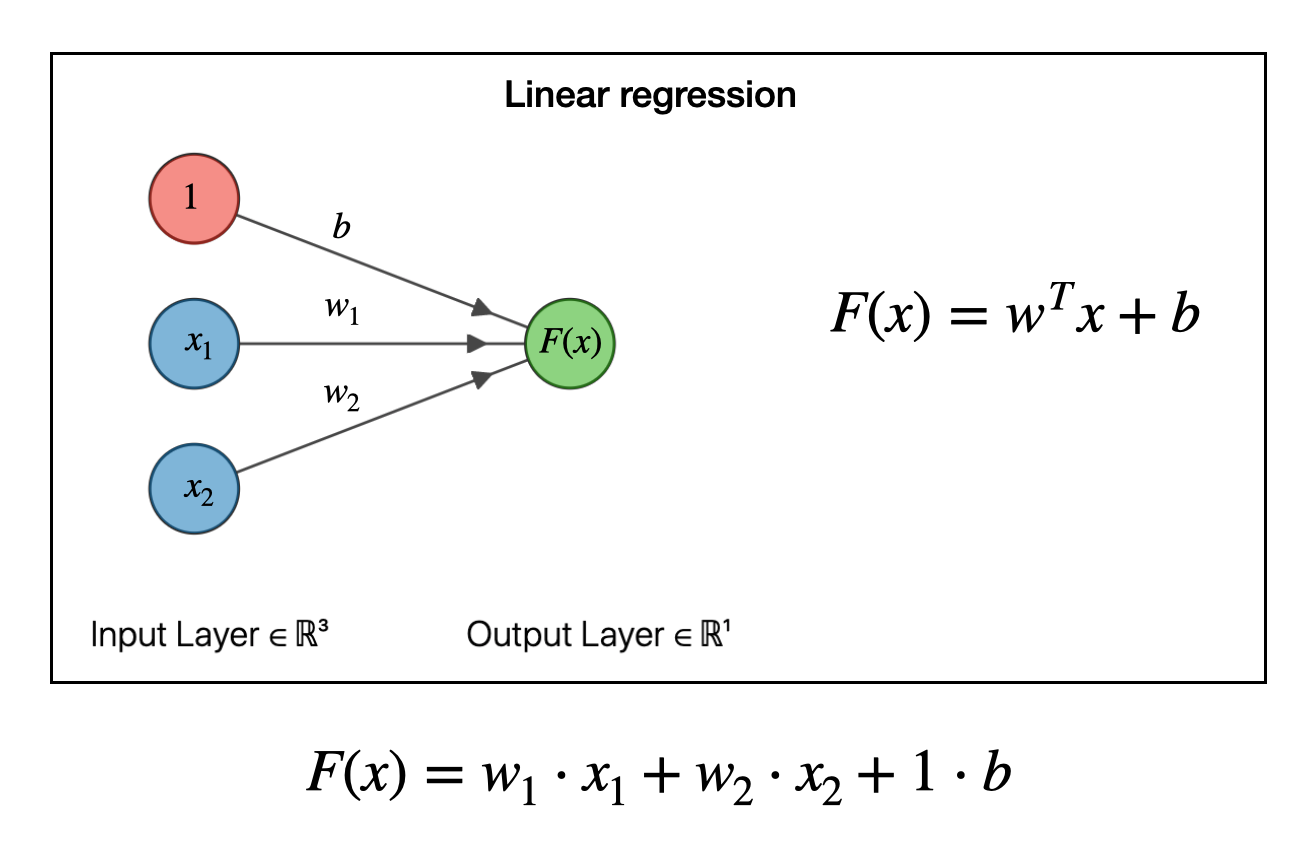
\includegraphics[width=0.85\textwidth]{linear.png}
    \caption{Linear combination of basis functions $\phi_j(x)$ weighted by parameters $w_j$.}
    \label{fig:linear_basis}
\end{figure}
\subsubsection*{Different Basis Functions}

\begin{itemize}
    \item \textbf{Polynomial Basis Function:}
    \begin{equation*}
    \phi_j(x) = x^j
    \end{equation*}

    \item \textbf{Gaussian Basis Function:}
    \begin{equation*}
    \phi_j(x) = \exp \left\{ -\frac{1}{2} \left( \frac{x - \mu_j}{s} \right)^2 \right\}
    \end{equation*}
    where $\mu_j$ is the location parameter or center of the $j$-th basis function in the input space. It controls where along the $x$-axis the specific basis function is activated. The parameter $s$ is the scale parameter (often related to the variance $\sigma^2$ or standard deviation $\sigma$ of Gaussian). It governs the width or spread of the basis function.

    \item \textbf{Sigmoid Basis Function:}
    \begin{equation*}
    \phi_j(x) = \sigma \left( \frac{x - \mu_j}{s} \right)
    \end{equation*}
    where $\sigma(a)$ is the logistic sigmoid function:
    \begin{equation*}
    \sigma(a) = \frac{1}{1 + e^{-a}}
    \end{equation*}
    The function $\tanh(a) = 2\sigma(2a) - 1$ is similar to the logistic sigmoid.
\end{itemize}

\begin{figure}[h]
    \centering
    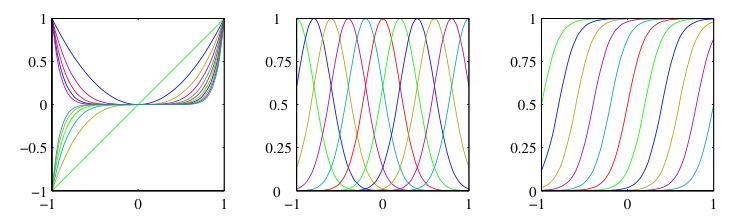
\includegraphics[width=0.85\textwidth]{basis-functions}
    \caption{Here is the image of Polynomial basis function, Gaussian Basis Function and Sigmoid Basis Function}
    \label{fig:linear_basis}
\end{figure}
\section{Mathematical Formulation of Linear Regression}

Linear regression learns a mapping $f : \mathcal{X} \to \mathcal{Y}$ from input features to output target variables. For $n$ training samples with $d$ features, let:
\begin{itemize}
    \item $X \in \mathbb{R}^{n \times d}$ be the design matrix (input features)
    \item $Y \in \mathbb{R}^n$ be the target vector
    \item $w \in \mathbb{R}^{d \times 1}$ be the weight vector
    \item $b \in \mathbb{R}$ be the bias term
\end{itemize}

The model hypothesis is:
\begin{equation*}
f(x) = w^T x + b
\end{equation*}

\subsection*{Loss Function}

The objective is to find $w$ that minimizes the error function $E(w)$:
\begin{equation*}
E(w) = \|Xw - Y\|^2 = (Xw - Y)^T (Xw - Y)
\end{equation*}

Expanding the matrix multiplication:
\begin{equation*}
E(w) = w^T X^T X w - w^T X^T Y - Y^T X w + Y^T Y
\end{equation*}

Now let's look at the middle terms:
\begin{align*}
w^T X^T Y &\implies (1 \times d) \times (d \times n) \times (n \times 1) = (1 \times 1) \quad \text{(a scalar)} \\
Y^T X w &\implies (1 \times n) \times (n \times d) \times (d \times 1) = (1 \times 1) \quad \text{(a scalar)}
\end{align*}

Using the scalar transpose identity (any scalar is equal to its own transpose, $\alpha = \alpha^T$):
\begin{equation*}
(w^T X^T Y)^T = Y^T (w^T X^T)^T = Y^T (X^T)^T (w^T)^T = Y^T X w
\end{equation*}

So, $w^T X^T Y = Y^T X w$. Therefore:
\begin{equation*}
E(w) = w^T X^T X w - 2 w^T X^T Y + Y^T Y
\end{equation*}

To get the minimum error, we take the derivative with respect to $w$ and set it to zero.

From matrix calculus, $\nabla_w (w^T A w) = 2 A w$ for a symmetric matrix $A$. Here, let $A = X^T X$. Notice that $A$ is symmetric because:
\begin{equation*}
A^T = (X^T X)^T = X^T X = A
\end{equation*}

Taking the derivative gives:
\begin{equation*}
\frac{\partial E(w)}{\partial w} = 2 X^T X w - 2 X^T Y
\end{equation*}

Now we have two methods to solve for $w$:

\subsection*{Case 1: Closed-Form Solution}

Set the gradient $\nabla_w E(w) = 0$:
\begin{align*}
2 X^T X w - 2 X^T Y &= 0 \\
X^T X w &= X^T Y
\end{align*}

Assuming $X^T X$ is invertible:
\begin{equation*}
w^* = (X^T X)^{-1} X^T Y
\end{equation*}

\textbf{Note:} This method calculates the exact global minimum in a single operation. No learning rate or training epochs are needed.

\subsection*{Case 2: Iterative Gradient Descent}

When $X^T X$ is too large to invert efficiently (or $n$ is very large), update weights iteratively over epochs using a learning rate $\eta$:

\begin{enumerate}
    \item \textbf{Initialize:} Set $w^{(0)}$ (small random values).
    \item \textbf{Compute Gradient:} At step $t$, evaluate the gradient:
    \begin{equation*}
    \nabla_w E(w^{(t)}) = 2(X^T X w^{(t)} - X^T Y)
    \end{equation*}
    \item \textbf{Update Weight:}
    \begin{equation*}
    w^{(t+1)} = w^{(t)} - \eta \nabla_w E(w^{(t)})
    \end{equation*}
    \item \textbf{Repeat} for a fixed number of epochs or until it converges ($\|\nabla_w E(w)\| < \epsilon$).
\end{enumerate}

Finally, for a new input $x$, calculate the predicted value $\hat{y}$:
\begin{equation*}
\hat{y} = w^T x + b
\end{equation*}

\section{Algorithmic Implementations}

To bridge theoretical derivations with software execution, the procedural logic for both optimization techniques is detailed below.

\subsection*{Algorithm 1: Closed-Form Solution (Normal Equations)}

\begin{algorithm}[H]
\caption{Closed-Form Linear Regression Solver}
\label{alg:closed_form}
\begin{algorithmic}[1]
\Require Design Matrix $X \in \mathbb{R}^{n \times d}$, Target Vector $Y \in \mathbb{R}^{n \times 1}$
\Ensure Optimal Weight Vector $w^* \in \mathbb{R}^{d \times 1}$
\Procedure{NormalEquations}{$X, Y$}
    \State $A \gets X^T X$ \Comment{Compute $d \times d$ Gram matrix}
    \State $b \gets X^T Y$ \Comment{Compute $d \times 1$ target projection}
    \If{$\det(A) = 0$} 
        \State $A^{-1} \gets $ Pseudo Invert Matrix $X^T X$ 
    \EndIf
    \If{$\det(A) \neq 0$} 
    		\State $A^{-1} \gets \text{Invert}(A)$ \Comment{Invert $d \times d$ matrix via LU/Cholesky}
    \EndIf
    \State $w^* \gets A^{-1} \cdot b$ \Comment{Compute parameters $w^* = (X^T X)^{-1} X^T Y$}
    \State \Return $w^*$
\EndProcedure
\end{algorithmic}
\end{algorithm}

\vspace{1em}

\subsection*{Algorithm 2: Iterative Batch Gradient Descent}

\begin{algorithm}[H]
\caption{Batch Gradient Descent Linear Regression}
\label{alg:gradient_descent}
\begin{algorithmic}[1]
\Require $X \in \mathbb{R}^{n \times d}$, $Y \in \mathbb{R}^{n \times 1}$, Learning rate $\eta > 0$, Tolerance $\epsilon > 0$, Max Epochs $K$
\Ensure Optimized Weight Vector $w \in \mathbb{R}^{d \times 1}$
\Procedure{GradientDescent}{$X, Y, \eta, \epsilon, K$}
    \State Initialize $w^{(0)} \sim \mathcal{N}(0, 0.01 \cdot I_{d \times 1})$ \Comment{Small random initial weights}
    \State $t \gets 0$
    \Repeat
        \State $\hat{Y} \gets X w^{(t)}$ \Comment{Compute predictions for all $n$ samples}
        \State $E \gets \hat{Y} - Y$ \Comment{Compute error residual vector}
        \State $g^{(t)} \gets 2 \cdot X^T E$ \Comment{Compute gradient $\nabla_w E(w) = 2(X^T X w - X^T Y)$}
        \State $w^{(t+1)} \gets w^{(t)} - \eta \cdot g^{(t)}$ \Comment{Update weight parameters}
        \State $t \gets t + 1$
    \Until{$\|g^{(t)}\|_2 < \epsilon$ \textbf{or} $t \ge K$} \Comment{Convergence check}
    \State \Return $w^{(t)}$
\EndProcedure
\end{algorithmic}
\end{algorithm}

\end{document}